% \title{Teil 2: Infrastrukturen der Metrologie: 
% Akkreditierung, DAkkS}
% \author{Dozent: Dr.-Ing. Gerd Ehret \\ Physikalisch-Technische Bundesanstalt}
% \date{21. Jan. 2019}
% \begin{document}
% \maketitle
% \begin{centering}
% 	\Large{Teil 2 zur Zwölften Vorlesung zu} \\[1ex] 
% 	\Large{\textbf{Messdatenauswertung und Messunsicherheit (MDA)}} \\[2ex]
%	\large{Modulverantwortlicher:} \\
%	\large{Prof. Dr.-Ing. R. Tutsch, iprom, TU Braunschweig}\\
% \end{centering}
\section{Internationale Metrologieorganisationen (BIPM,NMIs)}
...
\section{Akkreditierung, Zertifzierung, DAkkS}
\subsection{Messen, Prüfen, Lehren}
\textbf{Messen:} Ermittlung von Werten einer Messgröße i.~Allg. unter festgelegten Bedingungen (Messbedingungen), siehe z.~B. auch die Definition von \textit{Messung} im \cite{VIM08}

\textbf{Prüfen:} Ermittlung von Eigenschaften (quantitative, qualitativ) eines Objektes nach einem vorgegebenen Verfahren - häufig auch einschl. Vergleich mit vorgegebenen Spezifikationen (\textit{Konformität}) Prüfen bedeutet nach DIN 1319 das Feststellen, inwieweit ein Prüfobjekt eine Forderung erfüllt \cite{DIN1319}. Wird nur mit dem menschlichen Sinnen – ohne Hilfsmittel – geprüft, spricht man vom subjektiven Prüfen. Die Prüfergebnisse sind nur schlecht miteinander vergleichbar. Werden Hilfsmittel – sogenannte Prüfmittel – verwendet, so spricht man vom objektiven Prüfen.

\textbf{Lehren:} Objektive Prüfverfahren werden in die Arten Messen und Lehren unterteilt. Beim Messen wird eine physikalische Größe mit einem Messgerät erfasst und ein Messwert ermittelt. Der Messwert setzt sich aus Zahlenwert mit Einheit, welche die physikalische Größe repräsentiert, zusammen. Beim Lehren wird festgestellt, ob das zu prüfende Objekt innerhalb vorgegebener Grenzen liegt oder nicht. Das \textit{Prüfergebnis ist kein Zahlenwert, sondern eine Gut- / Schlecht-Aussage}. Oft lässt sich beim Lehren erkennen, in welche Richtung die Grenze überschritten wurde. 

\subsection{Akkreditierung (Wirtschaft)}
Die Anforderungen an die Qualität von Waren und Dienstleistungen nehmen angesichts der Liberalisierung des Welthandels sowie der steigenden Ansprüche von Verbrauchern, Unternehmen und Gesetzgebern stetig zu. Ob im Umweltschutz, in der Lebensmittel- oder Elektroindustrie, im Gesundheitswesen oder im Bereich Erneuerbarer Energien – in diesen wie in vielen anderen Wirtschaftsbereichen sind objektive Prüfungen, Kalibrierungen, Inspektionen oder Zertifizierungen daher von großer Bedeutung \cite{wiki01}.

Diese Bewertungen stellen sicher, dass die überprüften Produkte, Verfahren, Dienstleistungen oder Systeme hinsichtlich ihrer Qualität und Sicherheit \textit{verlässlich} sind, sie einem technischen Mindestniveau entsprechen und mit den Vorgaben entsprechender Normen, Richtlinien und Gesetze konform sind. Daher werden diese objektiven Bestätigungen auch als Konformitätsbewertung bezeichnet.
Vertrauen durch Akkreditierung

Das Vertrauen in Zertifikate, Inspektionen, Prüfungen oder Kalibrierungen steht und fällt jedoch mit der Kompetenz desjenigen, der die Bewertungsleistung erbringt. Viele dieser sogenannten \textbf{Konformitätsbewertungsstellen} belegen die Qualität ihrer eigenen Arbeit daher durch eine Akkreditierung.

In diesem Verfahren weisen sie gegenüber einer unabhängigen Akkreditierungsstelle nach, dass sie ihre Tätigkeiten fachlich kompetent, unter Beachtung gesetzlicher sowie normativer Anforderungen und auf international vergleichbarem Niveau erbringen. Die Akkreditierungsstelle begutachtet und überwacht dabei das Managementsystem und die Kompetenz des eingesetzten Personals der Konformitätsbewertungsstelle.

Akkreditierungen tragen deshalb somit entscheidend dazu bei, die Vergleichbarkeit von Konformitätsbewertungsergebnissen zu gewährleisten und \textit{Vertrauen in die Qualität und Sicherheit von Produkten und Dienstleistungen zu erzeugen}.

Der Begriff \glqq Akkreditierung \grqq ~(Latein: \glqq accredere\grqq, Glauben schenken) wird in verschiedenen Bereichen benutzt, um den Umstand zu beschreiben, dass eine allgemein anerkannte Instanz einer anderen das Erfüllen einer besonderen (nützlichen) Eigenschaft bescheinigt. 

Akkreditierung im hier gemeinten Sinne ist gemäß ISO/IEC 17011:2005 definiert. Sie ist die Bestätigung durch eine dritte Stelle, die formal darlegt, dass eine Konformitätsbewertungsstelle (z.B. Laboratorien, Inspektions- und Zerti\-fizierungs\-stellen) die Kompetenz besitzt, bestimmte Konformitätsbewertungsaufgaben durchzuführen.

Konformitätsbewertungsstellen sind Organisationen, die folgende Dienstleistungen zur Konformitätsbewertung bereitstellen: Prüfung, Inspektion, Zertifizierung von Managementsystemen, Personen Personenzertifizierung im Sinne eines Qualifikationsnachweises und Produkten. \textbf{Kalibrierlabors} werden ebenfalls dem Begriff Konformitätsbewertungsstellen untergeordnet (obwohl sie nicht in erster Linie eine Konformität bewerten).

Eine \textbf{Zertifizierungsstelle} ist akkreditiert, wenn eine Akkreditierungsstelle formell bestätigt, dass die Zertifizierungsstelle die z.B. in der Normenreihe EN 45011–45013 aufgeführten Voraussetzungen zur Durchführung von Bewertungen von Managementsystemen (zum Beispiel Qualitätsmanagement oder Umweltmanagement), Produkten oder Personen erfüllt.
Ein\textbf{ Prüf- bzw. Kalibrierlaboratorium} ist akkreditiert, wenn es die z.~B. Anforderungen der Norm  DIN EN ISO/IEC 17025 erfüllt, die den Qualitätsstandard (DIN EN ISO 9001:2008) einschließt und darüber hinausgehende Anforderungen enthält. Hierzu wird das Labor durch eine \textbf{Expertengruppe} einer unabhängigen Akkreditierungsstelle, welche die Norm DIN EN ISO/IEC 17011 erfüllt, begutachtet und durch meist jährliche Begehungen überwacht.
Eine \textbf{Konformitätsbewertungsstelle} ist akkreditiert, wenn sie den Anforderungen z.~B. der Norm ISO/IEC 17021 (vormals ISO/IEC 45012) entspricht und eine Akkreditierungsstelle dies formell bestätigt.
Eine \textbf{Inspektionsstelle} ist akkreditiert, wenn sie die Anforderungen der Norm z.~B. ISO/IEC 17020 erfüllt und eine Akkreditierungsstelle dies formell bestätigt.

Beispiel: Die Akkreditierung von TÜV, DEKRA und Co \newline
Die TÜV-Gesellschaften, DEKRA und Co bekommen für ihre Arbeit eine sogenannte Akkreditierung von einer staatlichen Stelle namens DAkkS (Deutsche Akkreditierungsstelle), die bestätigt, dass die Messungen korrekt durchgeführt werden. Es kann durchaus mal passieren wie im
Jahre 2015, dass diese Akkreditierung bei Vorliegen von 
Fehlverhalten (hier: keine volsständige Dokumentation) die Akkreditung entzogen werden kann (siehe z.~B. Artikel: http://www.autobild.de/artikel/tuev-dekra-und-co-ohne-zulassung- -8471909.html)

In Deutschland ist seit dem 1. Januar 2010 ausschließlich die Deutsche Akkreditierungsstelle GmbH (DAkkS) für die Erteilung und Aufrechterhaltung von Akkreditierungen zuständig. Die Errichtung einer nationalen Akkreditierungsstelle erfolgte nach der Vorgabe der Verordnung (EG) Nr. 765/2008 und nach Maßgabe des deutschen Akkreditierungsstellengesetzes.
Gesellschafter der DAkkS sind zu gleichen Teilen die Bundesrepublik Deutschland, die Bundesländer und die durch den Bundesverband der Deutschen Industrie (BDI) vertretene Wirtschaft (siehe \cite{DAkkS}).

\textbf{Wer kann sich akkreditieren lassen?}

Die DAkkS akkreditiert Konformitätsbewertungsstellen (KBS). Als solche Stellen gelten Laboratorien, Zertifizierungs- und Inspektionsstellen, Anbieter von Eignungsprüfungen und Referenzmaterialhersteller (siehe Abb.\ref*{fig:Typen_von_KBA}).  
Die Akkreditierung einer KBS durch die DAkkS ist möglich, wenn diese die Anforderungen der entsprechenden internationalen Normen erfüllt.
\begin{figure}[!htp]
	\begin{center}
		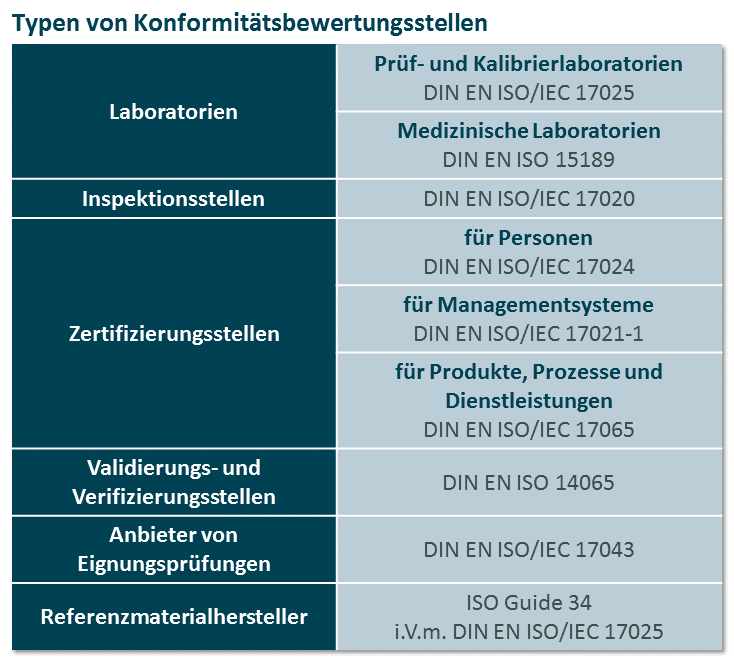
\includegraphics[width=120mm]{12_vorlesung/media/TypenKBS.png}
		\caption{Typen von Konformitätsstellen, Quelle:\cite{DAkkS} }
		\label{fig:Typen_von_KBA}
	\end{center}
\end{figure}

Die internationale Harmonisierung dieser Normen gewährleistet, dass die Akkreditierung weltweit nach gleichen Voraussetzungen erfolgt. Durch diese harmonisierten Normen und dank internationaler Abkommen werden die Bewertungsleistungen der in Deutschland akkreditierten Stellen in vielen anderen Ländern Europas und der Welt anerkannt.

Diese Überwindung technischer Handelshemmnisse erleichtert den Handel über Grenzen hinweg und stellt sicher, dass die Ergebnisse von Konformitätsbewertungen ohne eine erneute Überprüfung \textit{international akzeptiert} werden.
\newpage
\textbf{Vorteile von Akkreditierungen}\newline
Für Unternehmen:
\begin{itemize}
\item Höhere Akzeptanz von Produkten und Dienstleistungen erleichtert den Marktzugang bzw. ermöglicht diesen erst
\item Einmal geprüft, überall akzeptiert: Internationale Vergleichbarkeit und Anerkennung von Zertifikaten, Inspektionen, Prüfungen oder Kalibrierungen vermeidet Kosten durch mehrfache Bewertungen
\item Kompetenznachweis erleichtert die Auswahl eines passenden Dienstleisters für die Konformitätsbewertung von Waren und Dienstleistungen
\end{itemize}
Für akkreditierte Stellen: 
\begin{itemize}
\item objektiver Beleg für die Güte und Kompetenz der Tätigkeit einer Konformitäts\-bewertungs\-stelle nach internationalen Standards
\item Wettbewerbsvorteile gegenüber nicht akkreditierten Marktteilnehmern
\end{itemize}
Für Verbraucher:
\begin{itemize}
\item größeres Vertrauen der Verbraucher in die Qualität von Produkten und Dienstleistungen – trotz eines komplexen Weltmarkts
\item weniger Produktfehler oder Rückrufaktionen
\end{itemize}
Für den Gesetzgeber: 
\begin{itemize}
\item verbesserte Wettbewerbsfähigkeit der Wirtschaft durch den Abbau \item technischer Handelshemnisse
\end{itemize}
\textbf{Akkreditierungsprozess}
\begin{itemize}
	
\item Antragsphase \newline
Der Akkreditierungsprozess beginnt mit der Einsendung des Akkreditierungsantrages und der fachspezifischen Anlagen an die Zentrale Antragsbearbeitung (ZAB) der DAkkS in Berlin.
Optional können sich Kunden auch vorab in einem Vorgespräch in den Geschäfts\-stel\-len der DAkkS über ihre angestrebte Akkreditierung oder das Akkreditierungsverfahren im konkreten Fall informieren.
Die ZAB überprüft in Abstimmung mit der zuständigen Fachabteilung der DAkkS den Antrag. Dabei wird auch geprüft, ob eine Befugnis erteilende Behörde (BeB) in das Akkreditierungsverfahren eingebunden werden muss.
Nach einer erfolgreichen Antragsprüfung informiert der zugeteilte Verfahrensmanager die antragstellende Konformitätsbewertungsstelle (KBS) über das weitere Vorgehen.

\item Begutachtungsphase \newline
In der zweiten Phase des Akkreditierungsprozesses begutachtet die DAkkS durch ein Begutachterteam die technische Kompetenz und das Managementsystem der KBS. Zunächst prüfen die Begutachter die eingereichten Dokumente, dann findet zum vereinbarten Termin die Begehung vor Ort statt. Der Umfang und die Dauer der Begutachtung sind von der Größe der KBS, dem beauftragten Geltungsbereich (Scope) der Akkreditierung und der Komplexität des Verfahrens abhängig.
Die Ergebnisse werden in einem Begutachtungsbericht dokumentiert.
Festgestellte Abweichungen kann der Kunde durch entsprechende Korrekturmaßnahmen im Anschluss an den Begutachtungstermin innerhalb von zwei Monaten beheben. Diese werden nochmals überprüft und bewertet.

\item Akkreditierungsphase \newline
In dieser Phase bewertet ein Akkreditierungsausschuss (AkA) die Begutachtungsergebnisse und entscheidet über die Erteilung der Akkreditierung.
Die DAkkS bescheinigt den erfolgreichen Abschluss der Akkreditierungsphase durch den Akkreditierungsbescheid und die Akkreditierungsurkunde. Damit bestätigt die DAkkS der überprüften KBS die Erfüllung der entsprechenden Normen, Standards oder Gesetzen im Hinblick auf ihre Konformitätbewertungstätigkeiten – und damit ihre technische Kompetenz.
Die Akkreditierung wird anschließend im Verzeichnis der akkreditierten Stellen gelistet.
\item Überwachungsphase \newline
Eine Akkreditierung ist in der Regel für fünf Jahre gültig. Um den Kompetenznachweis auch innerhalb dieser Zeit sicherzustellen, erfolgen in festgelegten Intervallen zwei bis drei Überwachungen – je nachdem, ob es sich um ein Laboratorium, eine Inspektions-, Zertifizierungs- oder Verifizierungsstelle handelt.
Der Akkreditierungszyklus endet spät\-est\-ens nach fünf Jahren mit dem Auslaufen der Akkreditierung und bedarf dann einer Reakkreditierung.	
\end{itemize}
\textbf{Akkreditierungssymbol}\newline
Auf Antrag gestattet die DAkkS einer akkreditierten Stelle die Verwendung des DAkkS-Akkreditierungssymbols (siehe Abb.\ref{fig:SymbolDAkkS}). Zusammen mit der eindeutigen Registrierungsnummer weist es auf die erfolgreiche Akkreditierung hin. Durch die genehmigte Verwendung des Symbols können akkreditierte Stellen ihren Kunden die nachgewiesene Kompetenz signalisieren.
\begin{figure}[!htp]
	\begin{center}
		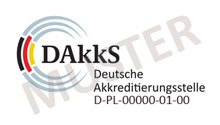
\includegraphics[width=60mm]{12_vorlesung/media/SymbolDAkkS.jpg}
		\caption{Muster des Akkreditierungssymbols der DAkkS für akkreditierte Stellen, Quelle:\cite{DAkkS} }
		\label{fig:SymbolDAkkS}
	\end{center}
\end{figure}

\textbf{Kosten der Akkreditierung} \newline
Als Deutschlands nationale Akkreditierungsstelle handelt die DAkkS zum Wohle des Staates, der Wirtschaft und der Verbraucher: Sie arbeitet im hoheitlichen Bereich kostendeckend, aber nicht gewinnorientiert.

\textbf{Gültigkeit von Akkreditierungen} \newline
Akkreditierungen sind üblicherweise fünf Jahre lang gültig, müssen jedoch in regelmäßigen Abständen durch die DAkkS überwacht werden.

\textbf{Änderungen in 2016: Eichbehören und PTB, 
DAkkS passt Regelung zur metrologischen Rückführung an}\newline
Die sogenannte „metrologische Rückführung“ ist eine der tragenden Säulen der Kon\-for\-mitäts\-bewertung. Die Deutsche Akkreditierungsstelle (DAkkS) hat ihre Regelungen zur Rück\-führungs\-politik nach Forderungen der Europäischen Kooperation für Akkreditierung (EA) angepasst. Danach ist ab August 2016 die Anerkennung von Rückführungsnachweisen, die von deutschen Eichbehörden ausgestellt wurden, nur noch in Einzelfällen möglich.Immer dann, wenn Messungen vorgenommen und die Messergebnisse für eine Kon\-formitäts\-bewert\-ung verwendet werden, ist die metrologische Rückführung von zentraler Bedeutung. Auf diesem Weg stellen Laboratorien und Inspektionsstellen die Richtigkeit der gemessenen Ergebnisse und der darauf basierenden Schlussfolgerungen – etwa die korrekte Einhaltung von Grenzwerten – sicher. Diese Stellen müssen daher im Rahmen eines Akkreditierungsverfahrens nachweisen, dass die Rückführung ihrer Messgeräte den internationalen Anforderungen entspricht.

Diese messtechnischen Anforderungen ergeben sich vor allem aus der Norm ISO/IEC 17025:2005 der Internationalen Organisation für Normung (ISO) sowie der verbindlichen Akkreditierungsregel ILAC P10:2013, die von der International Laboratory Accreditation Cooperation (ILAC) herausgegeben wird. Für alle durch die DAkkS akkreditierten Konformitätsbewertungsstellen sind diese Vorgaben in der DAkkS-Regel „Merkblatt zur messtechnischen Rückführung im Rahmen von Akkreditierungsverfahren“ (71 SD 0 005) zusammengefasst. Diese Regelung musste die DAkkS nun insbesondere im Hinblick auf die Rolle deutscher Eichbehörden anpassen.
In welchen Fällen sind Rückführungsnachweise deutscher Eichbehörden derzeit zulässig?

Die DAkkS-Regel 71 SD 0 005 zählt konkrete Möglichkeiten auf, wie Kon\-for\-mitäts\-bewertungs\-stellen gegenüber der DAkkS die Erfüllung der Anforderungen an die metrologische Rückführung nachweisen können. Eine bislang vorgesehene und praktizierte Möglichkeit bestand darin, einen Eichschein, Prüfschein oder Kalibrierschein einer deutschen Eichbehörde vorzulegen.

Voraussetzung dafür war bisher, dass die \textbf{ausstellende Eichbehörde} sich erfolgreich einem \textbf{Begutachtungsverfahren durch die Physikalisch-Technische Bundesanstalt (PTB), die metrologische Rückführung der relevanten Messgröße betreffend, unterzogen hat}. Dieses Vorgehen war aus Sicht der DAkkS, dem zuständigen Bundesministerium für Wirtschaft und Energie (BMWi) und der akkreditierten Konformitätsbewertungsstellen eine akzeptierte und praktikable Möglichkeit, den Nachweis der metrologischen Rückführung zu erbringen.

Warum wird sich die bisher gültige Regelung ändern?

Die europäische Akkreditierungsorganisation EA hat die Möglichkeit, Rückführungsnachweise von deutschen Eichbehörden unter gewissen Bedingungen zu akzeptieren, im Herbst 2014 bei der regelmäßig stattfindenden Evaluierung der DAkkS beanstandet, da Rückführungsnachweise ohne weitere Begutachtung durch die Akkreditierungsstelle nur dann anerkannt werden können, wenn die ausgebende Stelle den Rückführungsnachweis unter einer Akkreditierung erstellt hat. Eine Begutachtung durch die PTB allein ist hier nach dem internationalen Regelwerk (ISO/IEC 17025:2005) nicht ausreichend. Die DAkkS wurde im Oktober 2015 letztmalig aufgefordert, diese Regelung zu ändern.

EA hat diese Sichtweise am 28. Januar 2016 nochmals bestätigt, nachdem die DAkkS dagegen ein zulässiges Beschwerdeverfahren eingeleitet hatte. Als Folge dieser EA-Entscheidung hat die DAkkS in Abstimmung mit dem BMWi und der PTB die DAkkS-Regel 71 SD 0 005 überarbeitet und in der Revision 1.4 am 1. Februar 2016 veröffentlicht.

\subsection{Zertifizierung}

Als \glqq Zertifizierung \grqq~ (von lat. \glqq certe\grqq~ = bestimmt, gewiss, sicher und „facere“ = machen, schaffen, verfertigen) bezeichnet man ein Verfahren, mit dessen Hilfe die Einhaltung bestimmter Anforderungen nachgewiesen wird.

Zertifizierung ist ein Teilprozess der Konformitätsbewertung. Zertifizierungen werden oft zeitlich befristet von unabhängigen Zertifizierungsstellen wie z. B. DQS, TÜV oder DEKRA vergeben und die Standards unabhängig kontrolliert.

Anforderungsbereiche\newline
Die Bereiche, in denen Anforderungen gestellt werden, die zertifiziert werden können, umfassen im Allgemeinen:
\begin{itemize}
\item Produkte und Dienstleistungen und ihre jeweiligen Herstellungsverfahren einschließlich der Handelsbeziehungen
\item Personen
\item Systeme
\item Unternehmen
\end{itemize}

\textbf{Arten der Zertifizierung }
\begin{itemize}
\item Nachweis von Ausbildungsstandards oder besonders ausgearbeiteten Fachnormen bei Personenzertifizierungen. 
\item Nachweis von Ausbildungsstandards bei der Anerkennung von Ausbildungsinstituten, wie er beispielsweise durch Berufsverband|Berufsverbände durchgeführt wird (bei nichtuniversitären Ausbildungen wird teils von \glqq zertifizierten\grqq ~Ausbildungsinstituten, teils von \glqq akkreditierten\grqq ~Ausbildungsinstituten gesprochen, wobei Letztere zugleich befugt sind, Personenzertifikationen oder Teile davon durchzuführen).
\item International anerkannter Nachweis der persönlichen Befähigung, zum Beispiel als PMP (Project Management Professional) durch das PMI (Project Management Institute) IPMA-Zertifikate Level D-A für Projektmanager.
\item Zertifizierung eines Managementsystems (zum Beispiel nach ISO 9001, ISO 14001). 
\item Zertifizierung von Produkten oder Dienstleistungen. Für Zertifizierungsstellen, die Zertifizierungssysteme für Produkte oder Dienstleistungen betreiben, besteht die EN ISO/IEC 17065 (früher EN 45011 bzw. ISO/IEC Guide 65).
\item Zertifizierung der Herkunftsregion eines Produktes (DOC).
\item Zertifizierung der Informationssicherheit nach BS 7799 oder ISO 27001|ISO/IEC 27001.
\item Zertifizierung zum Nachweis der Einhaltung von Umwelt- und Sozialstandards, zum Beispiel bei der Zertifizierung von nachhaltig erzeugtem Holz (siehe Zertifizierung (Forstwirtschaft)|FSC) oder von Produkten aus Entwicklungsländern, die bessere Konditionen für die dortigen Produzenten garantieren nach Fairer Handel|Fair-Trade-Kriterien.
\item Zertifizierung zum Nachweis der Einhaltung von Anforderungen an den Arbeitssicherheit, Arbeits- und Umweltschutz gem. Occupational Safety and Health Administration|OHSAS bzw. ISO 14001
\item Zertifizierung zum Nachweis von Arbeitsbedingungen gemäß SA8000 und ähnlichen Regelwerken (Beispiele: Sedex und Business Social Compliance Initiative|BSCI).
\item In der Software-Industrie ist die Zertifizierung insbesondere im Hinblick auf die Computersicherheit wichtig:
\item Zertifizierung der Mitarbeiter zur Dokumentation von Fähigkeiten, Qualifikation und Kompetenz. Siehe dazu Liste der IT-Zertifikate.
\item Zertifizierung von Softwareprodukten in Hinblick auf Funktionalität und Qualität. Besonders wichtig sind hier der amerikanische TCSEC- und der Europäische Information Technology Security Evaluation Criteria-Standard sowie im Hinblick auf die internationale Anerkennung die Common Criteria (CC). In Deutschland erfolgt die Zertifizierung durch das Bundesamt für Sicherheit in der Informationstechnik|BSI.
\item Zertifizierung der IT-Umgebung nach IT-Grundschutz. Um in einem Unternehmen einen solchen Prozess zu begleiten, werden vom BSI Grundschutz-Auditoren lizenziert. Diese sind autorisiert, Testate als Vorbereitung auf die Zertifizierung auszugeben. Die eigentliche Zertifizierung erfolgt durch das BSI.
\item Im Bereich Linux und freie Software ist ein wichtiges zertifizierendes Institut das kanadische Linux Professional Institute|LPI.
\item In der Lebensmittelindustrie gibt es heute verschiedene Normen, angelehnt an die weltweit bekannte ISO 9001. Diese wurden zugeschnitten auf die Bedürfnisse der Lebensmittelindustrie. Weit verbreitete Standards sind zum Beispiel der International Food Standard (IFS), die Anforderungen des British Retail Consortium, Good Manufacturing Practice|GMP, Hazard Analysis and Critical Control Points und die ISO 22000. Zunehmender Akzeptanz erfreut sich für Fische auch der MSC-Standard des Marine Stewardship Council.
\item Packmittelhersteller, die Packmittel für den direkten Kontakt mit Lebensmitteln (Pri\-mär\-pack\-mit\-tel) herstellen, sind zunehmend nach der Norm BRC-IoP zertifiziert.
\item Zertifizierung von Altersvorsorgeprodukten, z. B. Riesterrente.
\item Zertifizierung von Energiemanagementsystemen gemäß ISO 50001.
\item Nachhaltigkeitszertifizierung von Biomasse und Biokraftstoffen.
\item Unternehmenszertifizierung, z.B. für den Bereich Nachhaltigkeit. Hier werden Standards vom Standardgeber vorgeschrieben. In diesem Fall wird vom Standardgeber definiert, was Nachhaltigkeit im unternehmerischen Kontext bedeutet. Das gesamte Unternehmen (Management, Lieferketten, Produkte usw.) wird im Zertifizierungsprozess überprüft.
\end{itemize}

\subsection{Konfirmitätsbewertung}
\glqq Konformitätsbewertung\grqq~ist in der internationalen Norm ISO/IEC 17000:2004 \glqq Kon\-for\-mitäts\-be\-wertung – Begriffe und allgemeine Grundlagen\grqq definiert als \glqq Darlegung, dass festgelegte Anforderungen bezogen auf ein Produkt, einen Prozess, ein System, eine Person oder eine Stelle erfüllt sind\grqq.

Konformitätsbewertung ist ein Überbegriff für Tätigkeiten des Auswählens, Ermittelns (von Eigenschaften), Bewertens (etwa auf Einhaltung vorgegebener oder allgemeiner Anforderungen) und Bestätigens (etwa durch Konformitätserklärung|Erklärung des Herstellers, oder ein Zertifizierung|Zertifikat einer Zertifizierungsstelle, dass ein Produkt bestimmte Normen einhält). Solche Tätigkeiten sind beispielsweise Stichprobennahme, Prüfen, Inspizieren, Erklären, Zertifizieren, Akkreditieren. Die Objekte der Konformitätsbewertung sind nicht eingeschränkt.

Konformitätsbewertung findet auf vielfältige Weise und allen Ebenen statt: 
\begin{itemize}
\item im Betrieb (etwa Endprüfung, Auditierung eines Qualitätsmanagementsystems durch eigene Auditoren):
\item durch Stellen / Personen des Kunden oder Abnehmers: 
\item durch kommerzielle, vom Auftraggeber unabhängige Konformitätsbewertungsstellen (etwa Laboratorien; Zertifizierungsstellen; Inspektionsstellen; Akkreditierung (Wirtschaft), Akkreditierungsstellen): 
\end{itemize}

EU-Konformitätsbewertung

Eine besondere Bedeutung hat die Konformitätsbewertung durch Benannte Stellen bei der Bewertung von Produkten auf ihre Übereinstimmung mit den Anforderungen einer Richtlinie (EU)|EU-Richtlinie. EU-Richtlinien gemäß Art. 95 EG-Vertrag für den Europäischer Binnenmarkt|Europäischen Binnenmarkt legen für zahlreiche Produkte Mindestanforderungen an die Sicherheit fest, die vom Hersteller erfüllt werden müssen.

Durch ein \glqq Konformitätsbewertungsverfahren\grqq~muss der Hersteller nachweisen, dass er die in der Richtlinie oder den Richtlinien enthaltenen grundlegenden Sicherheitsanforderungen eingehalten hat. Das Konformitätsbewertungsverfahren muss vom Hersteller für jedes Produkt vor dem erstmaligen Inverkehrbringen durchgeführt werden. Am Ende des Kon\-formitäts\-bewertungs\-verfahrens stellt der Hersteller eine EU-Konformitätserklärung für sein Produkt aus, in der er erklärt, dass das Produkt zu den Anforderungen der entsprechenden Richtlinie(n) konform ist. Am Produkt bringt der Hersteller dann die CE-Kennzeichnung an, falls die angewandte Richtlinie dies vorsieht.

Nur im Sektor \glqq Medizinprodukte\grqq~besteht die Besonderheit, dass im Rahmen der Konformitätsbewertung nicht nur die Produktsicherheit nachgewiesen werden muss, sondern zusätzlich auch die medizinisch-technische Leistungsfähigkeit von Medizinprodukten, so wie sie vom Hersteller in der Produktkennzeichnung einschließlich der Werbung als medizinische Indikation ausgelobt ist. Das entsprechende Nachweisverfahren nennt sich klinische Bewertung. Erst der (je nach der Produktklasse) extern durch Benannte Stelle zertifizierte Nachweis der Produktsicherheit und der Leistungsfähigkeit berechtigt Hersteller von Medizinprodukten zur Anbringung der \textbf{CE-Kennzeichnung}.

In den Anhängen der Richtlinien werden verschiedene Module für die Durchführung eines Konformitätsbewertungsverfahrens genannt. Welche Module gewählt werden können, hängt von der Klassifizierung des Produktes ab. Für Produkte mit höherem Risiko ist die Einbeziehung einer Benannten Stelle bei der Durchführung des Konformitätsbewertungsverfahrens obligatorisch.
Beispiele für Module:
\begin{itemize}
\item Modul A2: Interne Fertigungskontrolle durch den Hersteller und Überwachung der Abnahme durch benannte Stelle 
\item Modul B \textit{Baumusterprüfung}
EG-Baumusterprüfung (Feststellung der Übereinstimmung mit den einschlägigen internationalen und nationalen Fachnormen (DIN, EN, ISO, IEC etc.), IMO-Resolutionen und SOLAS-Bestimmungen)
\item Modul D
: Qualitätssicherung Produktion (Darlegung der Qualitätssicherungsmaßnahmen vor, während und nach der Produktion einschließlich deren Häufigkeit)
\item Modul E
: Qualitätssicherung Produkt (Darlegung der Qualitätssicherungsmaßnahmen nach der Produktion einschließlich deren Häufigkeit (Endabnahme und Prüfung))
\item Modul F
: Prüfung der Produkte (Prüfung der Produkte auf Übereinstimmung mit dem Baumuster entweder durch statistische Kontrollen oder Prüfung jedes einzelnen Produkts durch die Benannte Stelle)
\item Modul G
: Einzelprüfung (anwendbar auf Produkte, die nicht in Serie produziert werden)
\end{itemize}
Je höher das Gefahrenpotential eines Produktes ist, umso mehr Prüfungsumfang muss auf eine „Benannte Stelle“ übertragen werden. Diese wird durch eine vierstellige Kennziffer hinter der CE-Kennzeichnung angegeben. Die Konformitätsbewertung für Produkte mit einem sehr geringen Gefährdungspotenzial kann der Hersteller ohne Einschaltung einer Benannten Stelle selbst durchführen.

In jedem Fall - also auch bei Einschaltung einer Drittstelle - muss eine EU-Konformitätserklärung (in der Regel) durch den Hersteller ausgestellt werden. Dies unterstreicht dessen alleinige Verantwortung (= Haftung) für das Produkt.

Bei der Konformitätsbewertung müssen die Sicherheitsanforderungen der EU-Richtlinien eingehalten werden. 

\subsection{Audit}
Ein \glqq Audit\grqq~untersucht, ob Geschäftsprozesse, Anforderungen und Richtlinien die geforderten Standards erfüllen. Ein solches Untersuchungsverfahren erfolgt häufig im Rahmen eines Qualitätsmanagements. Die Audits werden von einem speziell hierfür geschulten Auditor durchgeführt.

Innerhalb des Qualitätsmanagements werden zwei Arten von Audits unterschieden: Im Bereich des Qualitätssicherung, statischen Qualitätsmanagements haben die Audits Prüfungscharakter, da sie  Nachweise über vertragsmäßige Vereinbarungen liefern. Sie werden daher pro Über\-prüfungs\-zyklus nur einmalig durchgeführt. In der Qualitätssicherung, dynamischen Qualitäts\-sicherung (oder Qualitätsmanagement) kommt den Audits eine erweiterte Bedeutung zu: Sie dienen der Erfassung von Entwicklungstrends und geben den Initiatoren von Veränderungen wichtige Rückmeldungen über die Wirksamkeit ihrer eingeleiteten Maßnahmen. Die Aussagekraft dieser begleitenden Audits steigt mit der Wiederholungsrate, mit der der identische Fragenkatalog der identischen Betroffenengruppe zum identischen Thema vorgelegt wird. Vorgaben macht die \glqq DIN/ISO 19011, Leitfaden zur Auditierung von Managementsystemen\grqq.

\subsection{DAkkS}
Wie bereits oben erwähnt ist die 
die \glqq Deutsche Akkreditierungsstelle GmbH\grqq ~(\glqq DAkkS\grqq) zuständig für Akkreditierungen. Sie ist die nationale Akkreditierungsstelle mit Sitz in Berlin.

Gründungsgeschichte \newline
Im Zuge der europäischen Verordnung (EG) Nr. 765/2008 (Artikel 4 Absatz 1) müssen alle EU-Mitgliedstaaten ab 1. Januar 2010 eine einzige nationale Akkreditierungsstelle benennen. Hierzu musste die Dachorganisation Deutscher Akkreditierungsrat (DAR) mit den folgenden vier Fachgesellschaften für bestimmte Gebiete zur DAkkS fusionieren:
\begin{itemize}
\item Deutsche Akkreditierungsstelle Chemie (DACH)
\item Deutscher Kalibrierdienst (DKD)
\item Deutsches Akkreditierungssystem Prüfwesen (DAP)
\item Trägergemeinschaft für Akkreditierung (TGA)
Über eine vorweggenommene Fusion enthält die TGA auch die Deutsche Akkreditierungsstelle Technik (DATech)
\end{itemize}
Organisation \newline
Die DAkkS ist eine privatwirtschaftliche Organisation, beliehene hoheitliche Aufgaben wahrnimmt. 

Die GmbH-Anteilseigner der DAkkS sind jeweils zu einem Drittel:
\begin{itemize}
\item die Bundesländer, vertreten durch die Länder Bayern, Hamburg, Niedersachsen, Nordrhein-Westfalen und Sachsen-Anhalt. 
\item die Bundesrepublik Deutschland, vertretend durch das Bundesministerium für Wirtschaft und Energie 
\item die Deutsche Wirtschaft, vertretend durch den Bundesverband der Deutschen Industrie (BDI). 
\end{itemize}
Die Bundesländer wurden primär beteiligt, um die bestehenden Organisationen der Länder leichter in die DAkkS zu überführen, \glqq wodurch parallele Strukturen und Aktivitäten auf Landesebene verzichtbar werden\grqq.

Kritik an der DAkkS: \textit{In einer gemeinsamen Erklärung kritisierten Eurolab-D, der Verband der Materialprüfungsanstalten (VMPA) e.V. und der Deutsche Verband Unabhängiger Prüf\-labor\-atorien (VUP) die vom Bundeswirtschaftsministerium (BMWi) vorgelegte Reform der Gebührenverordnung für die Akkreditierungsstelle. Die Preissteigerungsrate schade dem Mittelstand und somit dem Wirtschaftsstandort Deutschland.}

\begin{thebibliography}{------}
	\item[] \hspace*{5em}{\Large\bf zu Kapitel 12:}
%	\bibitem[Cox02]{Cox02} M. G. Cox: The evaluation of key comparison data, % Metrologia 39, 589-595 (2002)
  %  \bibitem[ISO13528]{ISO13528} ISO: Statistical methods for use in proficency %testing by interlaboratory comparison, Second edition 2015-08-01, corrected version 2016-10-15
   \bibitem[DIN1319]{DIN1319} DIN 1319 Teil 1, Ausgabe Januar 1995 Titel: Grundlagen der Messtechnik – Grundbegriffe. Herausgeber: DIN Deutsches Institut für Normung e.V. Beuth-Verlag GmbH, Berlin–Wien–Zürich.
    \bibitem[ISO17011]{ISO17011}ISO/IEC 17011:2005 
    \bibitem[VIM08]{VIM08} VIM International vocabulary of
    metrology – Basic and general
     concepts and associated terms (VIM) 3rd edition (2008)
    \bibitem[wiki01]{wiki01} https://de.wikipedia.org/wiki/Akkreditierung\_(Wirtschaft)
    \bibitem[DAkkS]{DAkkS} http://www.dakks.de
   \end{thebibliography}
\newpage
% % Die neue Fassung der weltweit gültigen Norm ISO/IEC 17025 für Laborakkreditierungen ist Ende November in englischer Fassung
% erschienen und enthält viele grundlegende Änderungen.  
% \section*{Anhang}
% \subsection*{A1: Herleitung }

% \newpage
% \section*{Übungsaufgaben}

